\subsection{FPGA Acceleration}

The main flow of MSM calculation in FPGA is shown in Figure \ref{fig:fpga-acceleration}. When performing MSM of a large number of curve points, we mainly use Pippenger's algorithm \cite{pip76} to reduce the calculation of point doubling in MSM calculation process to improve calculation efficiency. Then perform a point addition on the buckets we get from the calculation.

\begin{figure}[!ht]
    \centering
    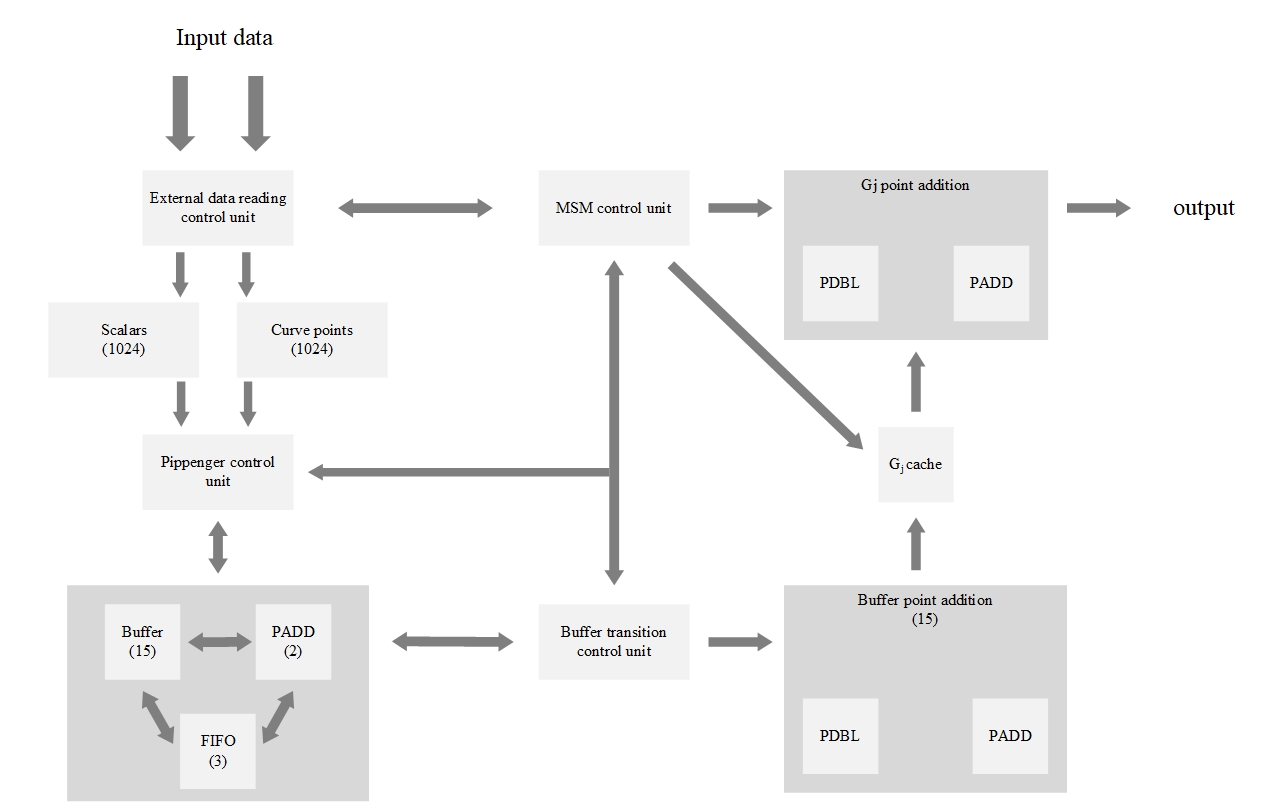
\includegraphics[width=0.8\textwidth]{fpga-acceleration.jpg}
    \caption{FPGA acceleration}
    \label{fig:fpga-acceleration}
\end{figure}

During the whole calculation process, we need a main control logic: MSM control logic, which completes the triggering of the external data reading logic, monitoring the status of the Pippenger control logic, Buffer transition and reading, point addition and point doubling control of the output results of Pippenger's algorithm. This is the brain of MSM.

The core process of the whole calculation is Pippenger's algorithm. In Pippenger's algorithm, firstly, read 1024 scalar values and 1024 curve points from the external memory through the external data reading control logic. Divide the scalar values into 4 bits, and then scan the curve points to complete PADD operation operation. It involves four modules in Pippenger's algorithm: the Pippenger control logic, Buffer, FIFO group and PADD operation. The Pippenger control logic mainly completes the division of sliding windows for scalar values, the cyclic extraction of curve point coordinates and the allocation, control of FIFO reading and writing, and the input and output of PADD. The Buffer buffers the output of PADD operation, while the FIFO group buffers the input of PADD operation.

Due to the limited on-chip memory of FPGA, Pippenger's algorithm can only perform MSM calculations of 1024 points each time. First up, extract the lowest 4 bits of the scalar values and perform point addition of 1024 points. After the addition operations, transfer the cache points in the Buffer, which requires the buffer transition control unit to complete. Secondly, after the point addition operations of 1024 scalars, the next Pippenger of 1024 points needs the Buffer transition control unit to load the Buffer point corresponding to the lowest 4 bits of last time. Then continue the operation, which will also be completed by the Buffer transition control unit.

After the point multiplication operations using Pippenger's algorithm, we need to perform point doubling and point addition operations on the result of the Buffer cache points we get from calculations. Finally, output the operation result of MSM.
